\documentclass{article}
\usepackage{graphicx}
\usepackage{algorithm}
\usepackage[noend]{algorithmic}
\usepackage{subfigure}
\usepackage{amssymb, amsmath, graphicx, charter, latexsym}
\usepackage{layouts}
\usepackage[letterpaper]{geometry}
\usepackage{enumerate}
\usepackage{epstopdf}
\usepackage{ragged2e}
%\usepackage{times}
\usepackage{mathtools}
%\usepackage[scaled]{helvet}
\usepackage{mathptmx}
\usepackage{verbatim}

\begin{document}

\title{ECEN 689: Real-Time Wireless Networks\\ Project 1, due on 2/26}
\date{}
\author{%
Ping-Chun Hsieh\\
UIN: XXXXXXXXXX\\
\texttt{lleyfede@tamu.edu}
\and
Tao Zhao\\
UIN: 825000452\\
\texttt{alick@tamu.edu}
\and
Dongni Han\\
UIN: XXXXXXXXXX\\
\texttt{handongni2015@tamu.edu}
}
\maketitle

\section*{Terminology}

In our report, we use ``server'' to denote the WiFi access point (AP), and
``client'' to denote the terminal device such as a mobile phone, a tablet, and
so on. Throughout our simulation, we let node $0$ be the server, and node $1$ be
the client, which correspond to the device A and B in the problem descriptions
respectively.

S-WiFi is the name of our application as well as our project. It stands for
Smart WiFi, or whatever you think it is.

\section{Downlink Transmissions}
\section{Uplink Transmissions with PCF}
\section{Transmission Reliability}

\begin{figure*}[h]
\centering
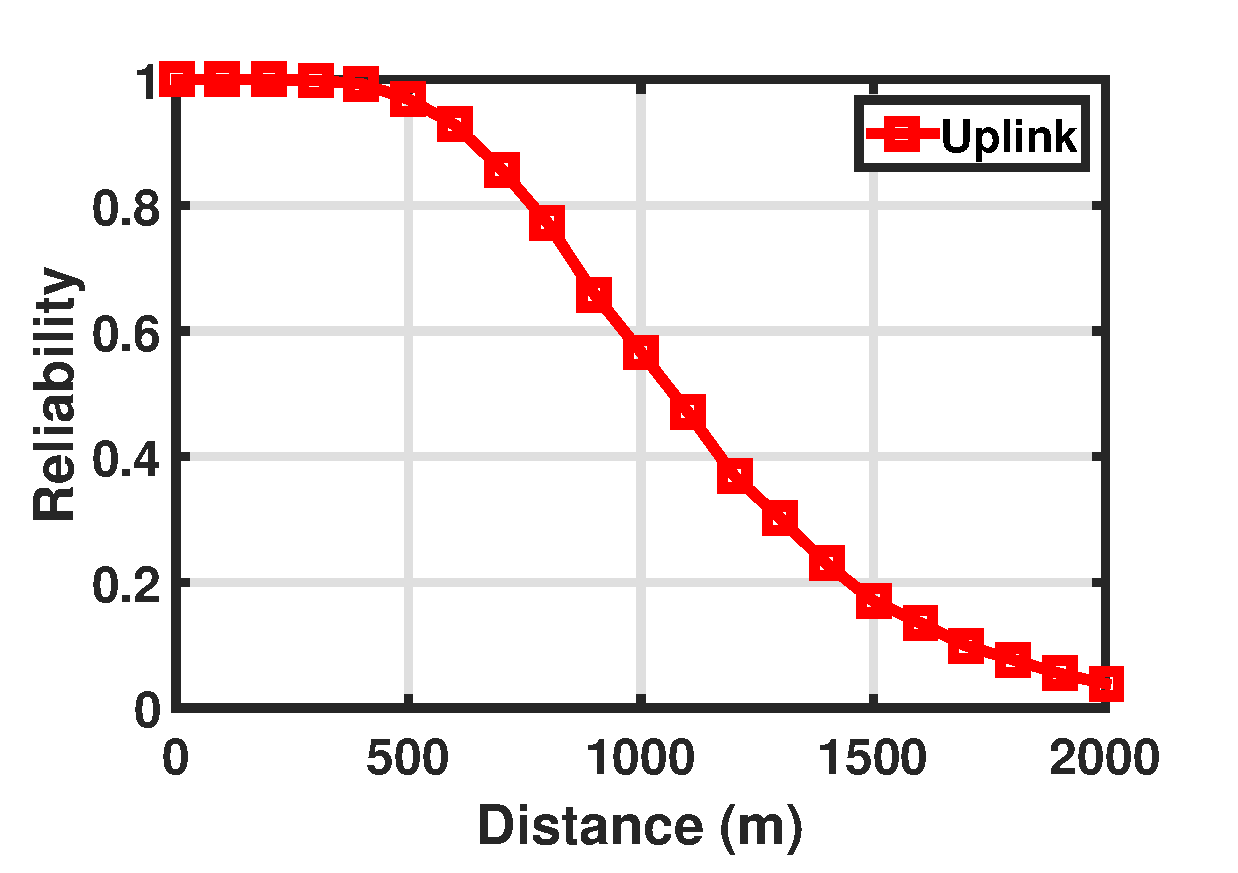
\includegraphics[width=3.5in]{p3_uplink.eps}
\caption{Reliability versus distance for uplink transmissions.}
\end{figure*}

\section{Measuring Delays}
\section{Preferences for Final Report}
We prefer topic 2 to topic 3, and prefer topic 3 to topic 1. ($2 \succ 3 \succ 1$)


\end{document}
